
\section{Experimental results}
\label{sec:exp}

{\em\color{gray} Need to present here both practical results that illustrates the outcome of our solution and how it benefits ... eg show a casewhere new goals are introduced as we go along}

{\em\color{gray} Also need some analysis -- potentially numerical -- on the overhead and impact fo both solutions relative to each other but also potentially to a more direct classic approach. 
To finally discuss why one solution was preferred on our system} 

\begin{figure}
  \centering
  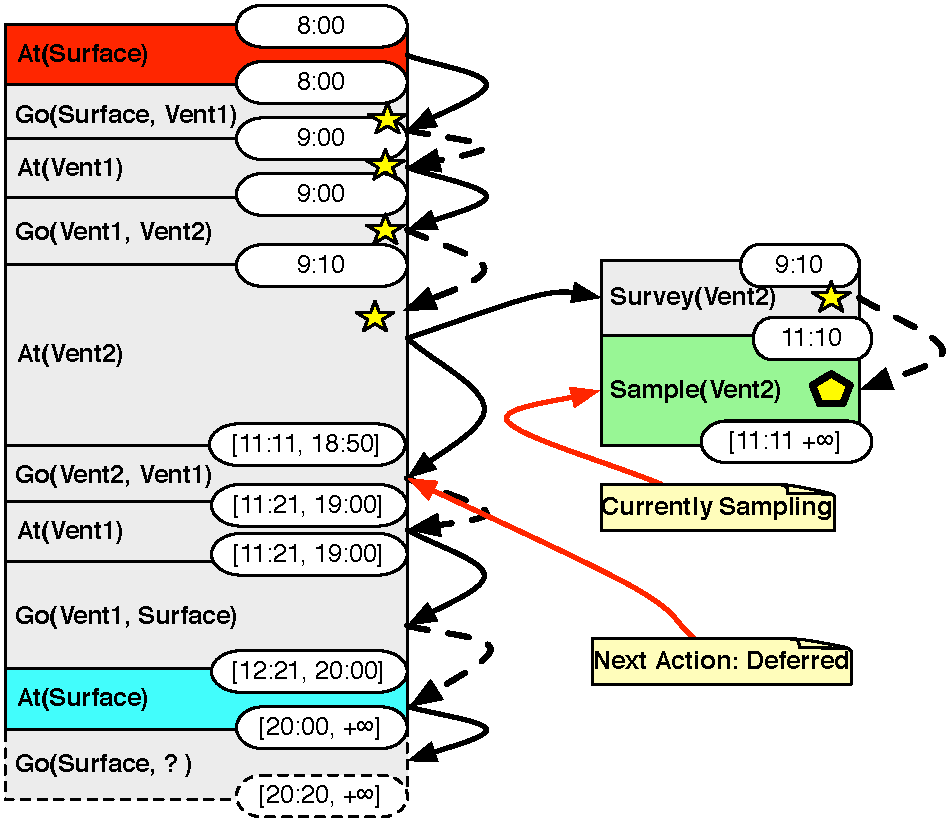
\includegraphics[width=0.8\columnwidth]{figs/example_MixedInitial}
  \caption{Our algorithm solution for the plan from Fig. \ref{fig:ex:plan}}
  \label{fig:ex:mixed1}
\end{figure}

\begin{figure}
  \centering
  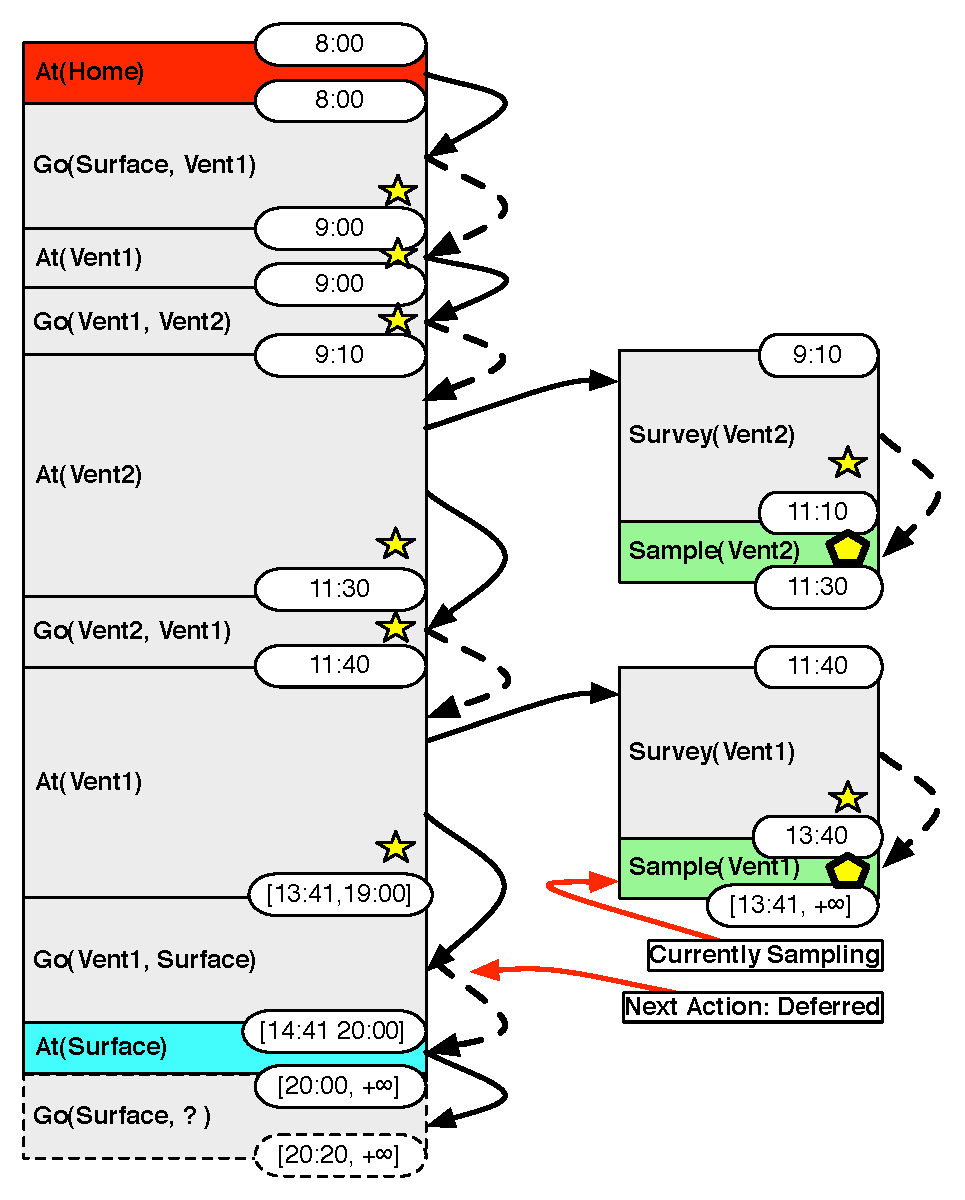
\includegraphics[width=0.8\columnwidth]{figs/example_MixedUpdate}
  \caption{Our algorithm solution after receiving external request for the plan from Fig. \ref{fig:ex:mixed1}}
  \label{fig:ex:mixed2}
\end{figure}



%%% Local Variables: 
%%% mode: latex
%%% TeX-master: "aaai13"
%%% End: 
